\documentclass[11pt, letterpaper]{report}
\usepackage{geometry}
\usepackage{graphicx}
\usepackage[spanish]{babel}
\usepackage{xcolor}
\definecolor{darkblue}{rgb}{0, 0, 0.5}
\usepackage[colorlinks=true,linkcolor=black,anchorcolor=black,citecolor=darkblue,filecolor=black,menucolor=black,runcolor=black,urlcolor=darkblue]{hyperref}
\usepackage[utf8]{inputenc}
\usepackage[T1]{fontenc} 
\usepackage{setspace}
\geometry{lmargin=3cm, rmargin=3cm, tmargin=2.65cm, bmargin=3cm}
\usepackage[pages=some]{style/background}
\usepackage{natbib}

\backgroundsetup{
	scale=1,
	angle=0,
	opacity=1,
	color=black,
	hshift=-159,
	contents={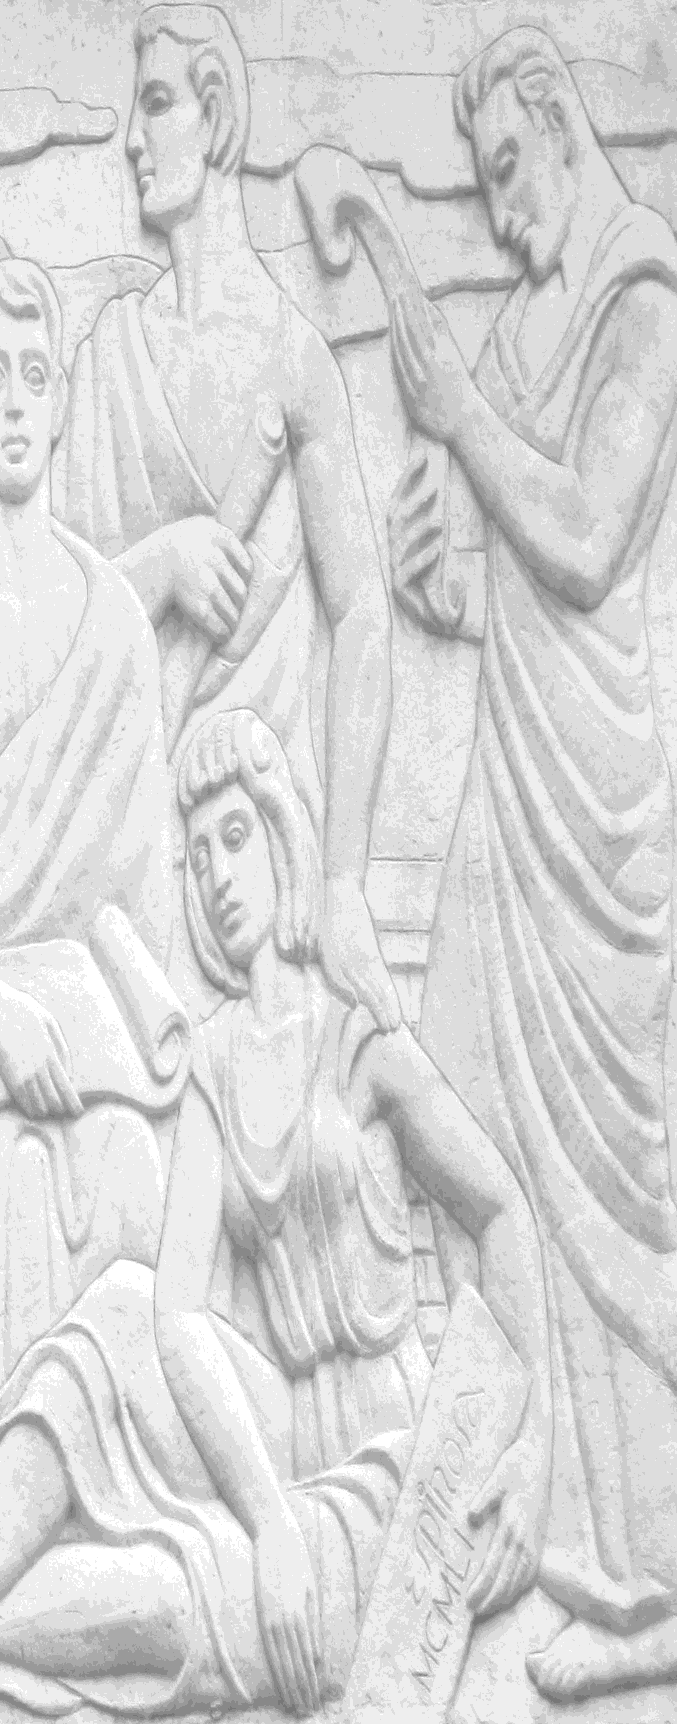
\includegraphics[width=0.48\paperwidth,height=\paperheight]{images/portada.png}}
}


\begin{document}
	\begin{titlepage}
	\begin{minipage}[t]{0.48\textwidth}
		\BgThispage
		\parbox{\textwidth}{}
	\end{minipage}
	\begin{minipage}[t]{0.55\textwidth}
			\parbox{\textwidth}{
				
\includegraphics[width=.8\textwidth]{images/logo.png}\\[0.5cm]
				\centering\textsc{Facultad de Ciencias Naturales y Exactas}\\[0.2cm]
				\centering\textsc{Departamento de Ciencia de la Computación}\\[2.2cm]
				\textbf{\LARGE Trabajo de Diploma en\\[-.1cm]Opción al Título de\\[-.1cm]Licenciado en Ciencia de la\\[-.1cm]Computación\\[2.2cm]}
				\Large  \textbf{Título}:\\
				\fontsize{18pt}{20pt}\selectfont Aprendizaje Profundo para el Perfilado de Usuarios en Redes Sociales\\
				\vspace{10mm}
				\begin{tabular}{rp{0.7\textwidth}}
					{\Large \bf Autor:} & {\Large Roberto Labadie Tamyao} \\[.5cm]
					{\Large \bf Tutores:} & {\Large Dr. Daniel Castro Castro} \\[.5cm]
					& {\Large M.Sc. Reynier Ortega Bueno} \\[.5cm]
				\end{tabular}
				
				\vspace{10mm}
				{\Large \textbf{Curso 2020-2021}}
			}
	\end{minipage}
	\end{titlepage}
	
	\pagenumbering{roman}
	\thispagestyle{empty} 
	\renewcommand{\contentsname}{Contenido} \tableofcontents
	
	\pagenumbering{arabic}
\addcontentsline{toc}{chapter}{Introducción}
\chapter*{Introducción}
Internet se define como la interconexión mundial de redes individuales operadas por el gobierno, la industria, el mundo académico y las partes privadas. En cuestión de muy pocos años, Internet se consolidó como una plataforma muy poderosa que ha cambiado para siempre la forma de comunicarse.  Esta manera tan simple y accesible de compartir datos, ha propiciado un desplazamiento de los entes sociales hacia el uso casi exclusivo de este medio.
\\
Un rol fundamental dentro de este universo comunicativo lo juegan las redes sociales donde de acuerdo al sitio DataReportal\footnote{\url{https://datareportal.com/}} a finales de 2020 existían más de 3.8 mil millones de usuarios de los 4.5 mil millones de personas conectadas a Internet, lo cual implica un crecimiento desmedido de la cantidad de datos multimodales que se genera a diario.
\\
El mundo del Big Data \citep{Riahi2018BigDA} en el cual nos sumerge este hecho, reporta una situación beneficiosa para el desarrollo de procesos sociales, en cuanto a la cantidad de información brindada por los usuarios . 
Estos procesos van desde estudios de marketing donde la retroalimentación a partir de opiniones permiten dirigir de manera efectiva la promoción hacia grupos sociales específicos, hasta aplicaciones en el área de la Interacción Humano-Computadora (\textit{Human-Computer Interaction }HCI), donde el conocimiento de las características físicas y psicológicas de las personas permite personalizar la interfaz de comunicación. Sin embargo un cúmulo de información tan significativo, se hace imposible de tratar en un espacio de tiempo razonable a menos que se haga de manera automatizada.
\\
Diversos estudios se han dirigido al diseño de métodos para manejar tal cantidad de información y realizar inferencias a partir de la misma, a la vez que han contribuido al desarrollo en ramas tales como el Procesamiento del Lenguaje Natural (\textit{Natural Langauage Processing} NLP) y Visión por Computadoras (\textit{Computer Vision} CV) en el área de la Inteligencia Artificial (\textit{Artificial Intelligence} AI).
\\ 
Dentro del NLP, la tarea de Perfilado de Autores (\textit{Author Profiling AP}) \citep{Rosso2019,article} se encarga específicamente de realizar un análisis de la información textual elaborada por una persona que permita establecer atributos y patrones de comportamiento para caracterizarla en cuanto a sexo, rango de edades o rasgos personales (e.g si la persona es extrovertida o no, ideología política). Sin embargo, para el AP el hecho de que la información recuperada de estos textos varíe enormemente en términos de su formato aun cuando proviene de la misma persona, sumado a que las secuencias texuales constituyen información digital no estructurada, hacen desafiante el proceso de analizarla y clasificarla automáticamente. 
\\
Inicialmente este tipo de tareas se desarrollaban sobre contenido generado en textos formales, periódicos, cartas o revistas, sin embargo determinar el perfil de una persona mediante el análisis de su cuenta en una red social ha tomado un gran auge en los últimos años \citep{rangel:2018,rangel:2019,f6032ffbacb14369b7a45d1ba9bd0b8c}.
 Las redes sociales además de haber logrado acelerar la comunicación entre las personas así como reunir varias formas del pensamiento individual en un mismo espacio, se han convertido en un medio donde se desarrollan procesos negativos tales como, la divulgación de discursos de odio \citep{rangel2021profiling}, \textit{bullying} o de noticias falsas \citep{rangel:2020}. Este hecho introduce nuevos retos al AP con tareas que involucran la detección de elementos altamente subjetivas como la ofensa, la toxicidad en el lenguaje y otros patrones psicológicos de comunicación que hacen más complejo el perfilado en relación a otras tareas.  
\\
 La mayor parte de los avances en el desarrollo de sistemas de AP han sentado sus bases dentro del ambiente académico, reuniendo estudios tanto de la Ciencia de la Computación como de la Lingüística. Algunas de las campañas de evaluación más importantes donde se han compartido tareas de este tipo son \textit{Plagiarism, Authorship and Social Software Misuse} PAN\footnote{https://pan.webis.de/} y \textit{Evaluation of NLP and Speech Tools for Italian} EVALITA\footnote{http://www.evalita.it/}, los que se han dirigido últimamente al análisis del genero textual de micro-blogging  con un enfoque multilingüe, empleado en medios sociales como Twitter\footnote{https://twitter.com/}.
\\
Tradicionalmente se han empleado dos tipos de acercamientos que han probado empíricamente ser efectivos para tratar el AP en redes sociales: los \textit{basados en estilo}  y los \textit{basados en contenido}. Las propuestas basadas en estilo se refieren al hecho de analizar como los autores se expresan cuando escriben, en cambio la basada en contenido se apoyan en el área temática del texto analizado. La mayor contribución de varios trabajos se ha basado en la selección de atributos que permitan medir el estilo autor y el contenido simultáneamente mediante el empleo de métodos de Aprendizaje de Máquina (\textit{Machine Learning} ML).
\\
Un proceso crítico en este tipo de propuestas es la selección de rasgos para representar vectorialmente los elementos del texto,  en el cual pueden ser eliminados elementos que ayuden al modelo a discernir entre una clase u otra, en el caso de tareas de clasificación, pero también se puede introducir información ruidosa y de igual forma afectar su desempeño. 
\\
\\
En los últimos años dentro del Machine Learning ha tenido un auge enorme el Aprendizaje Profundo (\textit{Deep Learning} DL) en las áreas de CV y NLP, estableciendo nuevos estados del arte en la mayoría de sus tareas \citep{electronics8030292}. Este auge estuvo condicionado por las capacidades de procesamiento de las nuevas computadoras y la cantidad de datos disponibles. Los modelos de DL han mostrado una gran habilidad para aprender representaciones de rasgos (\textit{features}) con un alto nivel de abstracción. Estas representaciones capturan elementos que son posiblemente omitidos mediante la extracción manual de features y que facilitan el proceso de inferencia de los propios modelos de DL y de los métodos más tradicionales de ML. 
\\
Dentro del AP también se ha introducido el Aprendizaje Profundo con resultados alentadores. Sin embargo la mayoría de los modelos alcanzan mejores resultados al analizar la tarea a la que se orienta el perfilado cuando se emplean para clasificar mensajes individuales en lugar del perfil completo, e.g., se desempeñan mejor en la tarea de detección de odio en un tweet que en la detección de un perfil que tiende a usar un discurso de odio. 
\\
Por otro lado, las necesidades que cubren las tareas de AP incluyen la no sensibilidad de los sistemas ante la variación del idioma en el que la persona postee un mensaje o escriba una carta, es por ello que urge la extensión de los modelos de AI propuestos al esquema multilingüe que predomina en redes sociales como Twitter. \\Este trabajo de tesis se enmarca en el perfilado de autores en redes sociales empleando técnicas de Aprendizaje Profundo para el modelado y la clasificación de los perfiles teniendo en cuenta el enfoque multilingüe propio de este medio. 

\addcontentsline{toc}{section}{Problemática}
\section*{Problemática}
La mayoría de los trabajos existentes que emplean DL para resolver tareas de perfilado de autores en redes sociales, tanto tradicionales (e.g., determinar rango de edades, sexo, etc.) como las más recientes (e.g. detección de divulgadores de discursos de odio en redes sociales o noticias falsas) ven afectado su desempeño al tratar con las secuencias muy largas que se pueden generar al analizar un perfil completo a la vez, en vez de mensaje a mensaje. La perdida de información (\textit{information vanishing}) en este tipo de secuencias en términos de relaciones a largo plazo que presentan las estructuras sintácticas del lenguaje, es la causa fundamental de esta dificultad. Por esta razón sería conveniente dividir el problema de ``clasificar un perfil'' en subproblemas y construir una arquitectura modular, en la que primero se modele el perfil y luego este sea clasificado.
\\
Por otro lado en Cuba existe un limitado tratamiento y aplicación de este tipo de métodos automatizados para llevar acabo tareas de impacto como las mencionadas, ya sea en el área forense o empresarial .

\addcontentsline{toc}{section}{Hipótesis}
\section*{Hipótesis}
Dividir el proceso de clasificación de un perfil dentro de una tarea en: (1) codificar los mensajes individualmente y (2) modelar-clasificar el perfil, puede ayudar a prevenir la perdida de información generada del análisis de largas secuencias. Esto sumado a la capacidad de representar la información no estructurada de los métodos de DL puede influir positivamente en la precisión de las predicciones.  Además, proponer un modelo lo suficientemente robusto, podría incentivar el empleo de esos métodos automatizados  de AP en nuestro país.

\addcontentsline{toc}{section}{Objetivos}
\section*{Objetivos}
\subsection*{Objetivo General}
Diseñar una arquitectura de Aprendizaje Profundo modular para resolver la tarea de Perfilado de Autores en redes sociales teniendo en cuenta un enfoque multilingüe.
\subsection*{Objetivos Específicos}
\begin{enumerate}
	\item Diseñar una arquitectura que capture rasgos abstractos que permitan clasificar un perfil de usuario de una red social atendiendo tanto a tareas relacionadas con características demográficas de los autores, como con aspectos psicológicos de los mismos.
	\item Extender la arquitectura propuesta a un enfoque multilingüe de las tareas evaluadas.
	\item Evaluar y analizar el empleo de arquitecturas modulares basadas en DL sobre colecciones de datos propuestas en tareas de AP compartidas en la plataforma PAN (2019, 2020, 2021).
\end{enumerate}
\section*{Estructura del Trabajo}
Este trabajo esta estructurado en tres capítulos además del introductorio y una última sección en la que se describen las conclusiones de las modelaciones y se proponen  caminos a seguir para trabajos futuros. Cada uno de los capítulos se listan a continuación: 

%%Poner la reerencia de cada capitulo cuando este listo
\begin{itemize}
	\item En el Capítulo 1 se describen de manera breve métodos del estado del arte así como conceptos básicos relacionados con el Machine Learning necesarios para la comprensión de este trabajo.
	\item El Capítulo 2 describe las tareas de AP en las que se evaluarán las arquitecturas propuestas, así como los datos anotados sobre los cuales se basan los procesos de entrenamiento y evaluación.
	\item En el Capítulo 3 se exponen los experimentos realizados en el proceso de ajuste de cada unos de los modelos y sus módulos sobre los lenguajes estudiados. 
\end{itemize}
. 
	\bibliographystyle{style/acl_natbib}
	\renewcommand{\bibname}{Referencias Bibliográficas}
	\bibliography{bibliography}
	
\end{document}